\documentclass[12pt, a4]{article}
\usepackage[english]{babel}
\usepackage[utf8x]{inputenc}
\usepackage{fullpage}
\usepackage{listings}
\usepackage{graphicx}
\usepackage{color}

%Syntax highlighting
\definecolor{blue-violet}{rgb}{0.54, 0.17, 0.89}
\definecolor{ao}{rgb}{0.0, 0.5, 0.0}
\definecolor{amaranth}{rgb}{0.9, 0.17, 0.31}
\definecolor{ballblue}{rgb}{0.13, 0.67, 0.8}
\definecolor{onyx}{rgb}{0.06, 0.06, 0.06}


\lstset{
  breaklines=true,                 % automatic line breaking only at whitespace
  captionpos=b,                    % sets the caption-position to bottom
  breakatwhitespace=false,
  keepspaces=true,
  numbers=left,
  numbersep=5pt,
  showspaces=false,
  showstringspaces=false,
  showtabs=false,
  tabsize=4,  
  backgroundcolor=\color{white},   % choose the background color
  commentstyle=\color{ao},    % comment style
  keywordstyle=\color{amaranth},    % keyword style
  stringstyle=\color{blue-violet},    % string literal style
  numberstyle=\tiny\color{ballblue},	   % number style
  basicstyle=\ttfamily\footnotesize\color{onyx} % size of fonts used for the code
}

%Document Header
\title{\textbf{Department of CSE\\SSN College of Engineering}}
\author{\textbf{Vishakan Subramanian - 18 5001 196 - Semester VII}}
\date{13 September 2021}

\begin{document}
\maketitle
\hrule
\section*{\center{UCS 1711 - Mobile Application Development Lab}}
\hrule
\bigskip

%Assignment Details
\subsection*{\center{\textbf{Exercise 5: Progress Bar and Alarm Clock using Multithreading}}}
\subsection*{\flushleft{Aim:}}
\begin{flushleft}
To develop Android applications for:
\begin{itemize}
	\item Progress Bar Simulation
	\item Simulation for Suspending the UI
	\item Alarm Clock
\end{itemize}

\bigskip
Use \textbf{multithreading} concepts to implement the progress bar.


\end{flushleft}

%Code
\newpage
\subsection*{\flushleft{Code - Progress Bar: Main Activity:}}
\begin{flushleft}
\lstinputlisting[language = Java]{ProgressBar/app/src/main/java/com/example/progressbar/MainActivity.java}
\end{flushleft}

%Code
\newpage
\subsection*{\flushleft{Code - Progress Bar: Main Activity Layout:}}
\begin{flushleft}
\lstinputlisting[language = XML]{ProgressBar/app/src/main/res/layout/activity_main.xml}
\end{flushleft}

%Output
\newpage
\subsection*{\flushleft{Output: Progress Bar:}}
\begin{figure}[h]
\centering
\caption{Output: Progress Bar.}
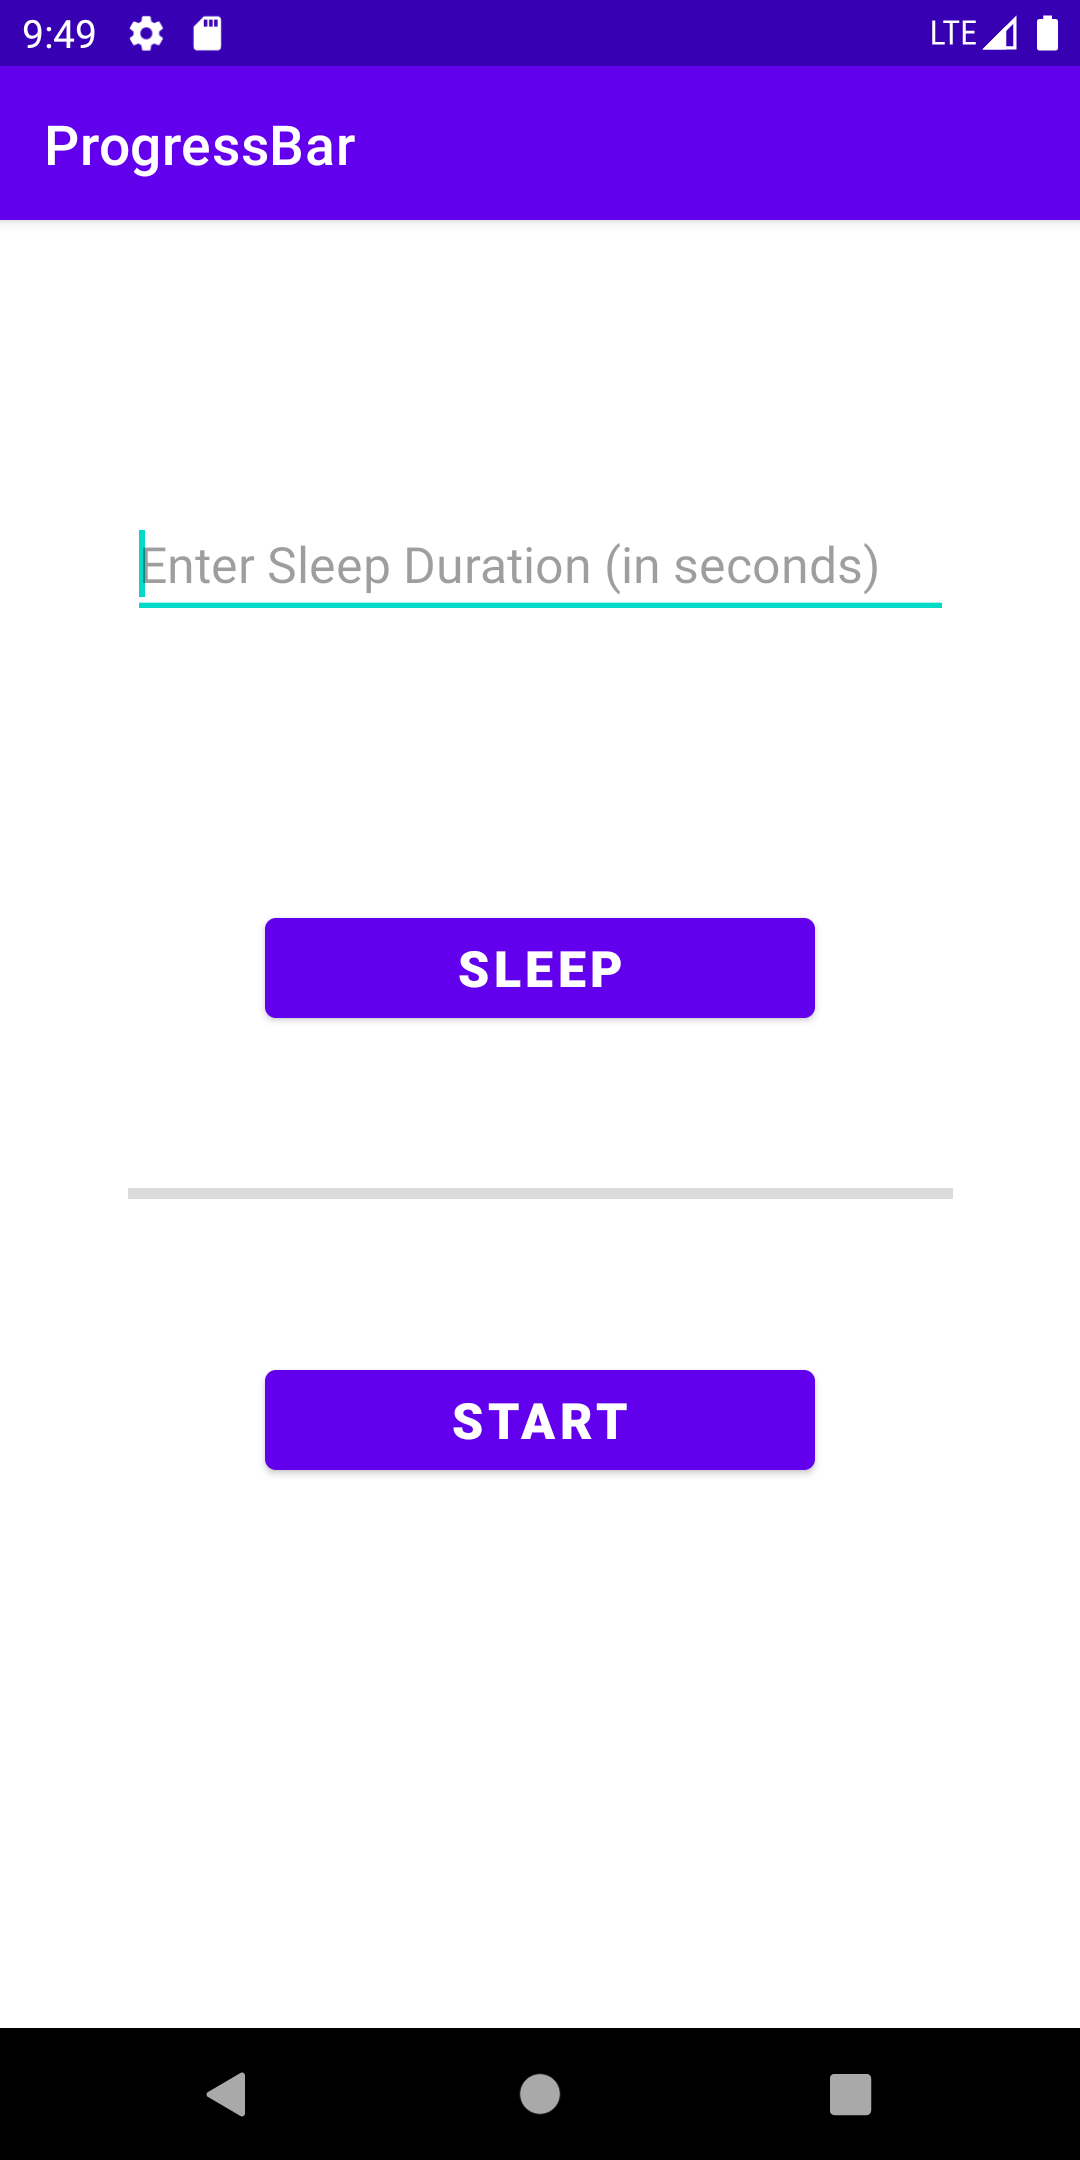
\includegraphics[height=15cm, width=7.3cm]{ProgressBar/Screenshots/Output-1.png}
\end{figure}

%Output
\newpage
\subsection*{\flushleft{Output: Progress Bar - Sleeping:}}
\begin{figure}[h]
\centering
\caption{Output: Progress Bar - Sleeping.}
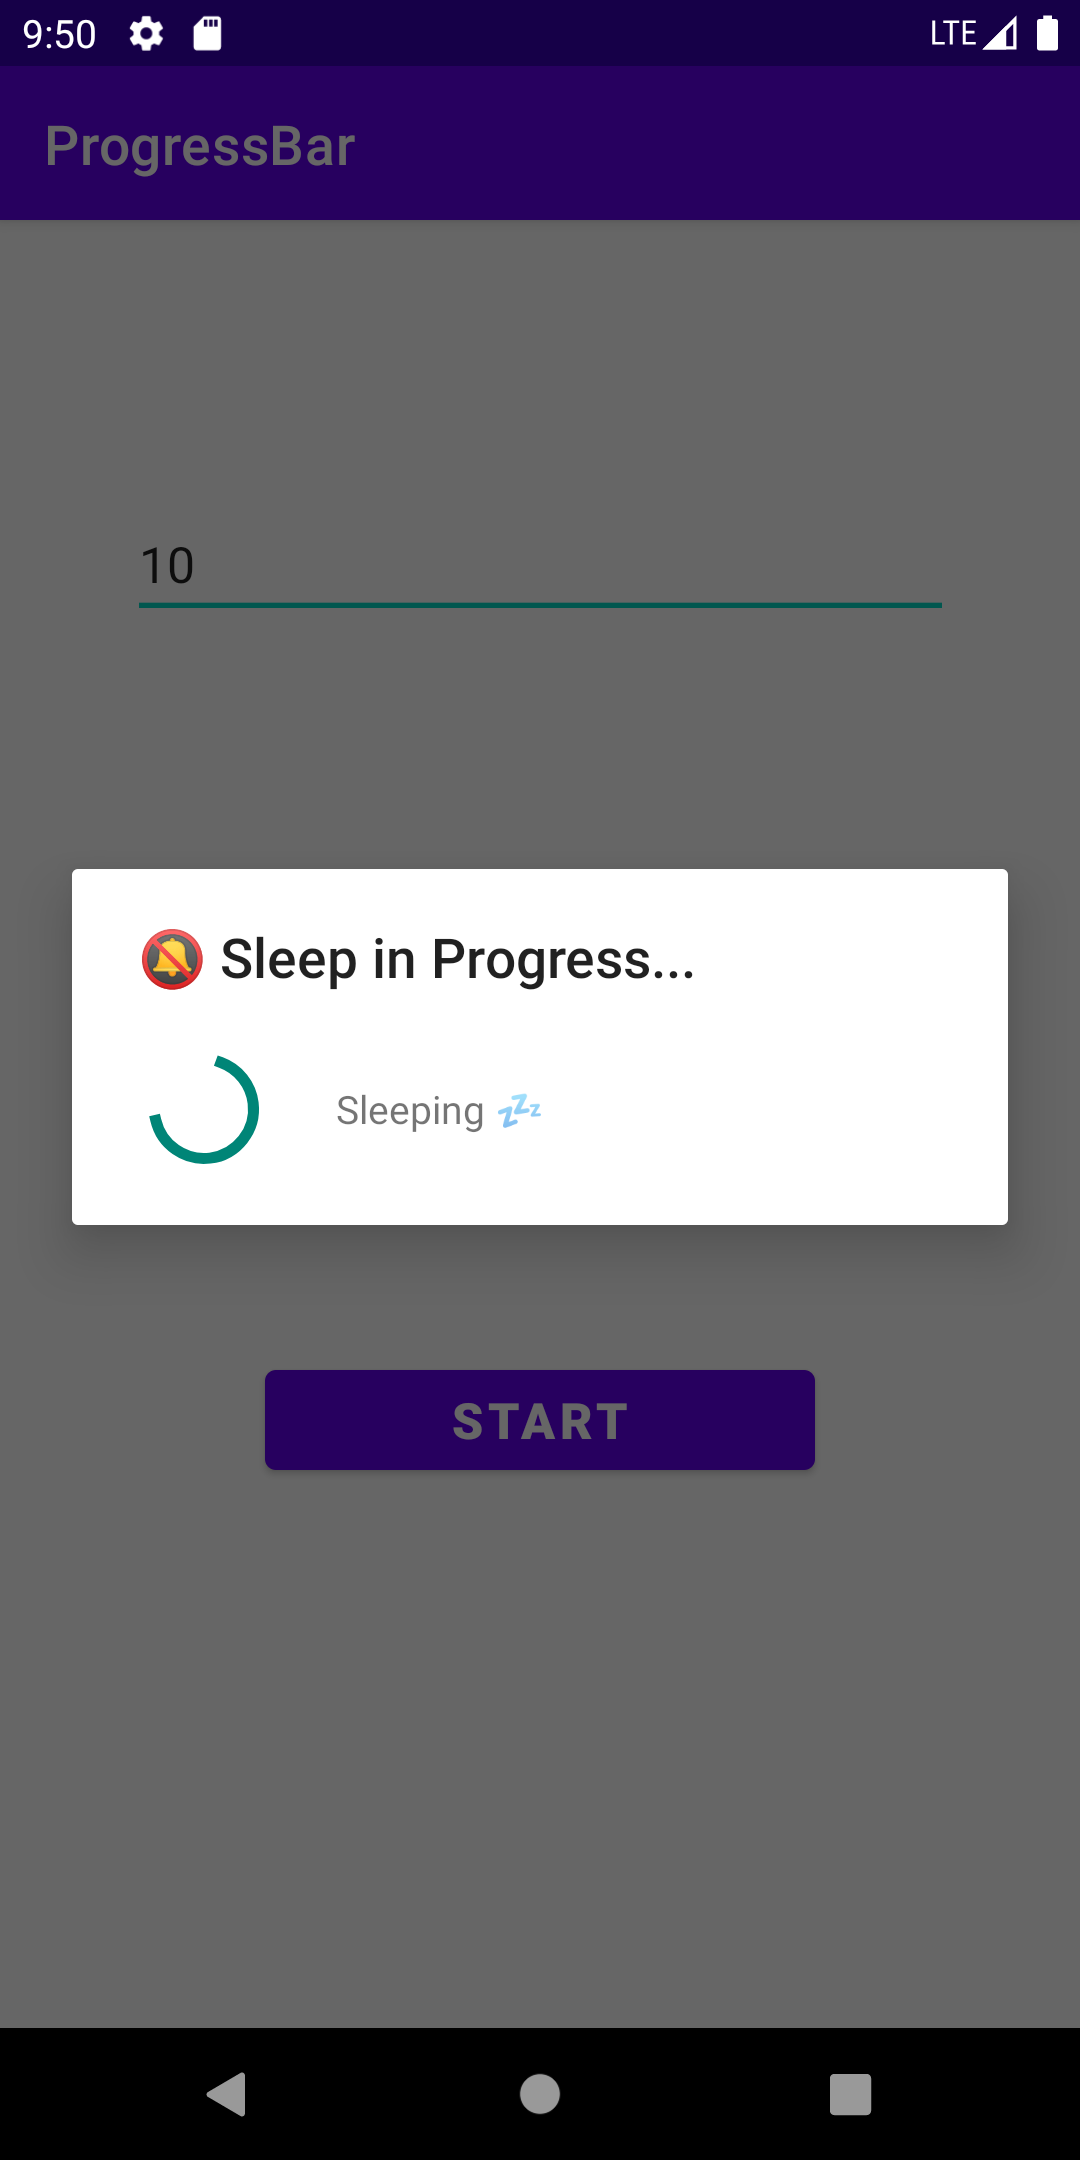
\includegraphics[height=15cm, width=7.3cm]{ProgressBar/Screenshots/Output-2.png}
\end{figure}

%Output
\newpage
\subsection*{\flushleft{Output: Progress Bar - In Progress:}}
\begin{figure}[h]
\centering
\caption{Output: Progress Bar - In Progress.}
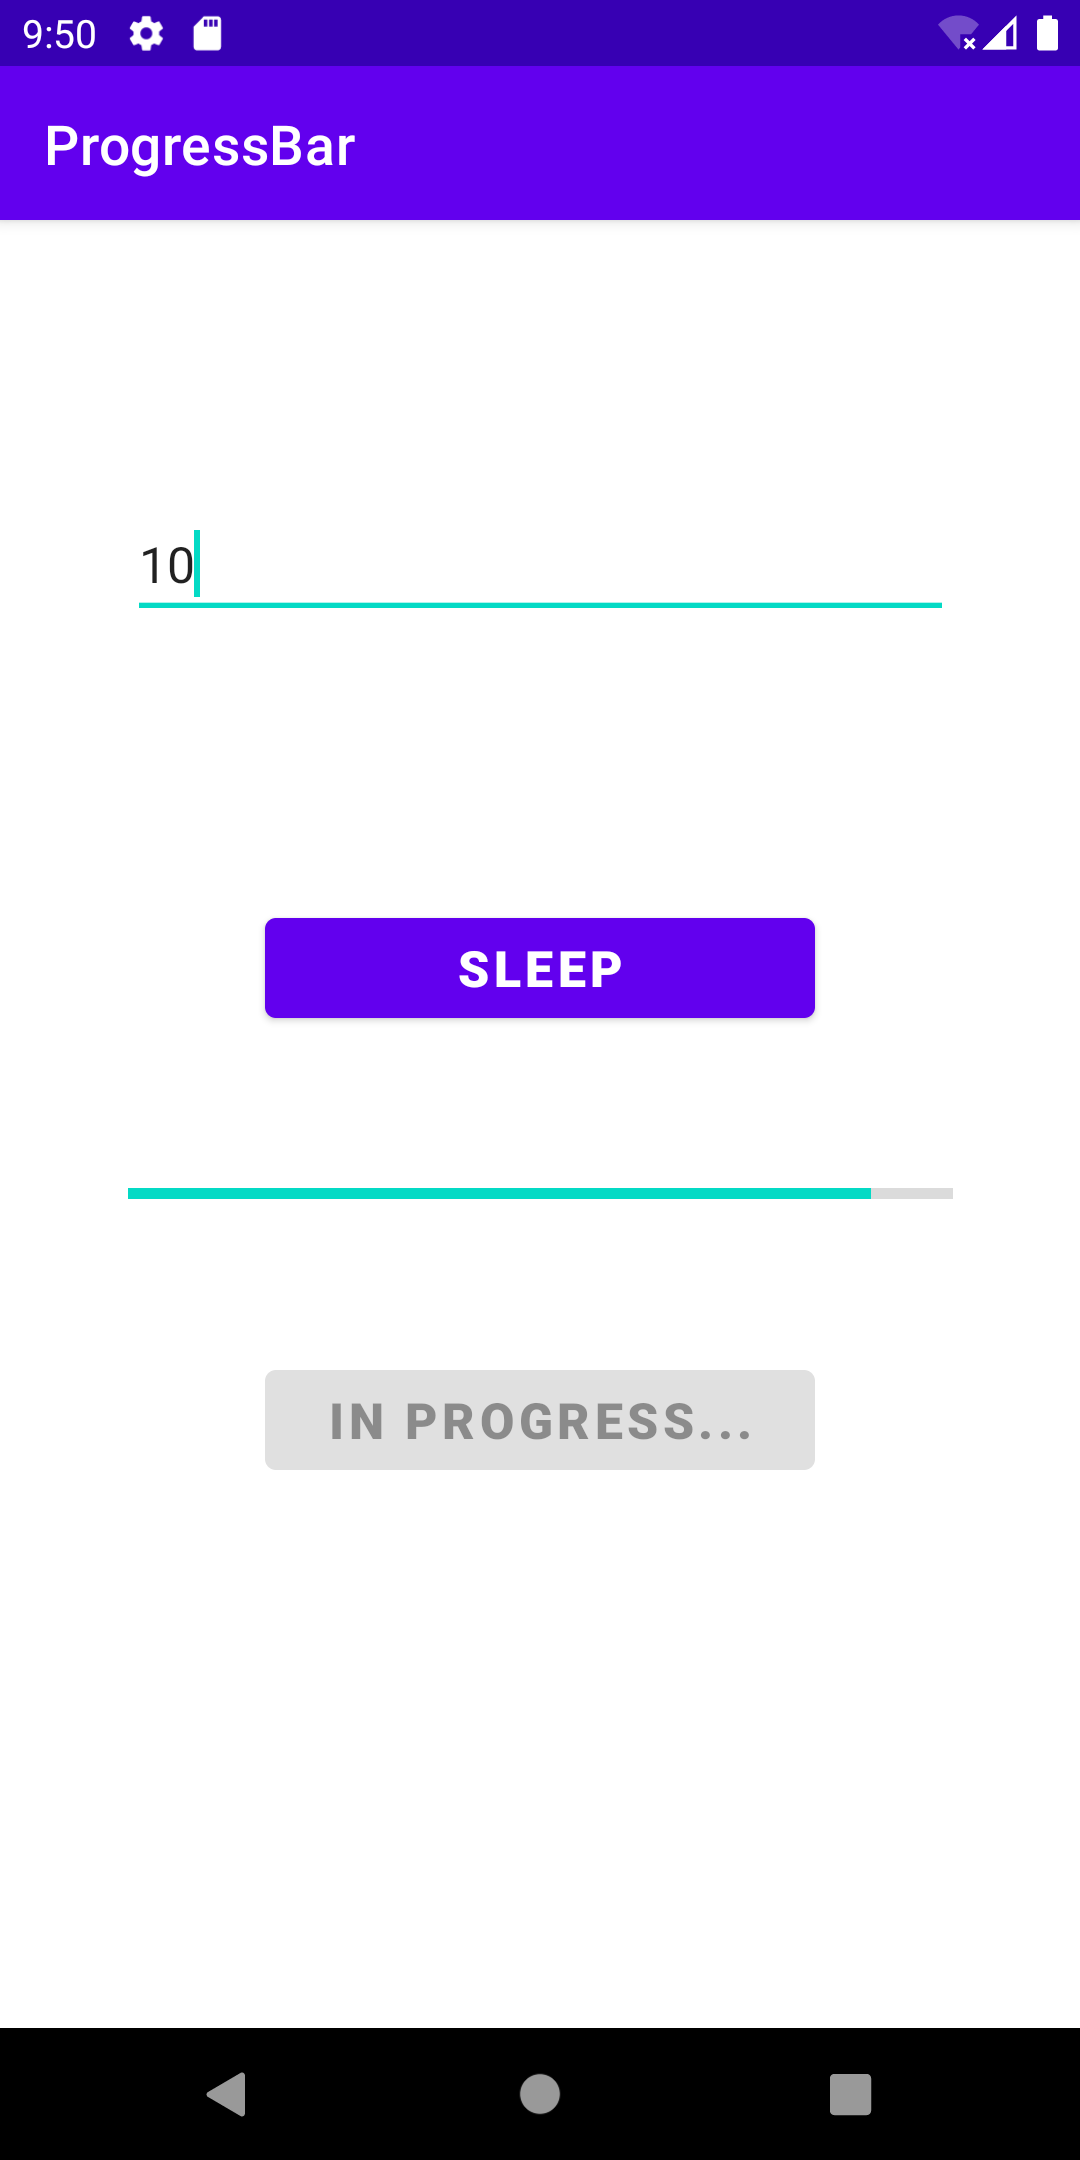
\includegraphics[height=15cm, width=7.3cm]{ProgressBar/Screenshots/Output-3.png}
\end{figure}


%Code
\newpage
\subsection*{\flushleft{Code - Alarm Clock: Main Activity:}}
\begin{flushleft}
\lstinputlisting[language = Java]{AlarmClock/app/src/main/java/com/example/alarmclock/MainActivity.java}
\end{flushleft}

%Code
\newpage
\subsection*{\flushleft{Code - Alarm Clock: Alarm Receiver Class:}}
\begin{flushleft}
\lstinputlisting[language = Java]{AlarmClock/app/src/main/java/com/example/alarmclock/AlarmReceiver.java}
\end{flushleft}

%Code
\newpage
\subsection*{\flushleft{Code - Alarm Clock: Main Activity Layout:}}
\begin{flushleft}
\lstinputlisting[language = XML]{AlarmClock/app/src/main/res/layout/activity_main.xml}
\end{flushleft}

%Code
\newpage
\subsection*{\flushleft{Code - Alarm Clock: Android Manifest XML:}}
\begin{flushleft}
\lstinputlisting[language = XML]{AlarmClock/app/src/main/AndroidManifest.xml}
\end{flushleft}

%Output
\newpage
\subsection*{\flushleft{Output: Alarm Clock:}}
\begin{figure}[h]
\centering
\caption{Output: Alarm Clock.}
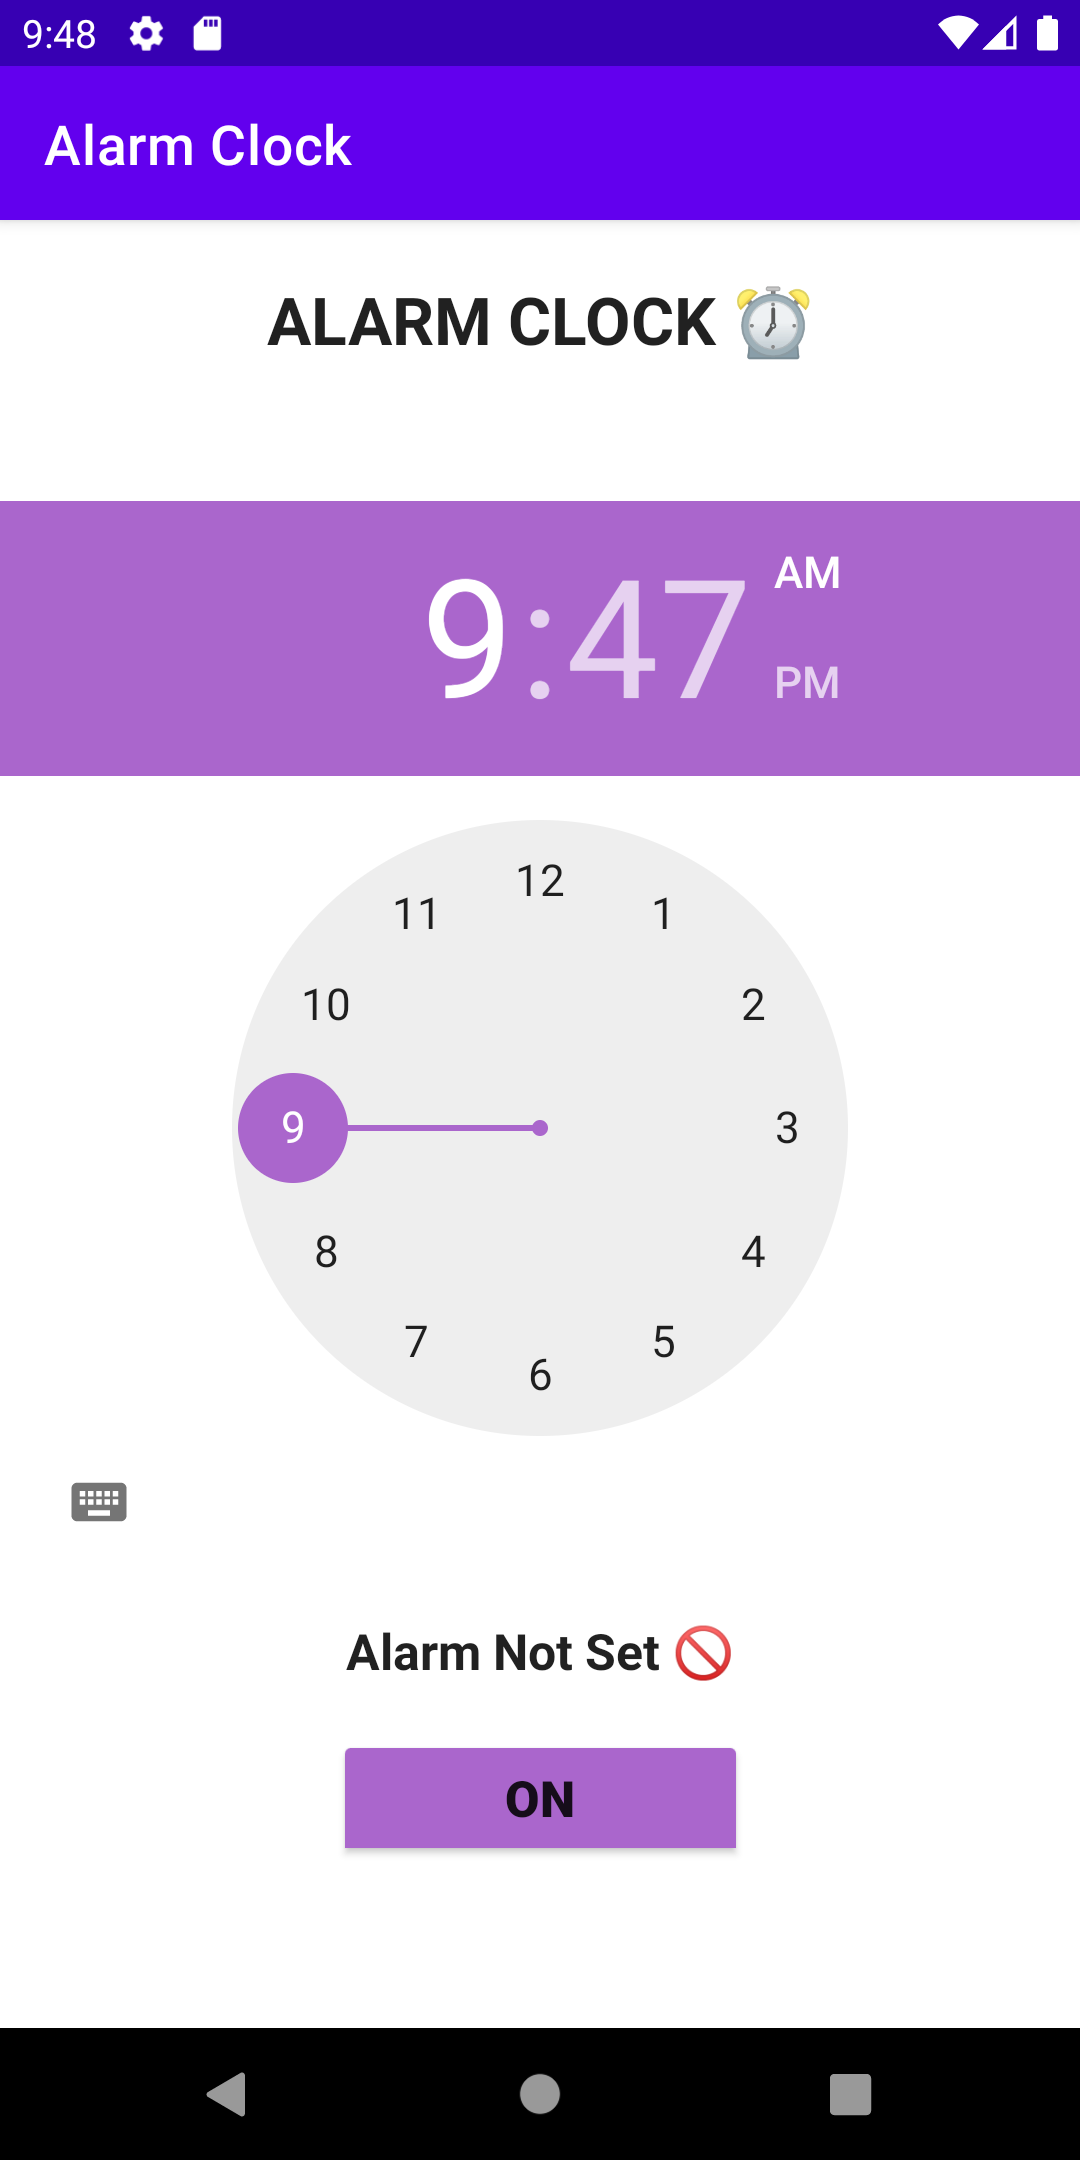
\includegraphics[height=15cm, width=7.3cm]{AlarmClock/Screenshots/Output-1.png}
\end{figure}

%Output
\newpage
\subsection*{\flushleft{Output: Alarm Clock - Alarm Set:}}
\begin{figure}[h]
\centering
\caption{Output: Alarm Clock - Alarm Set.}
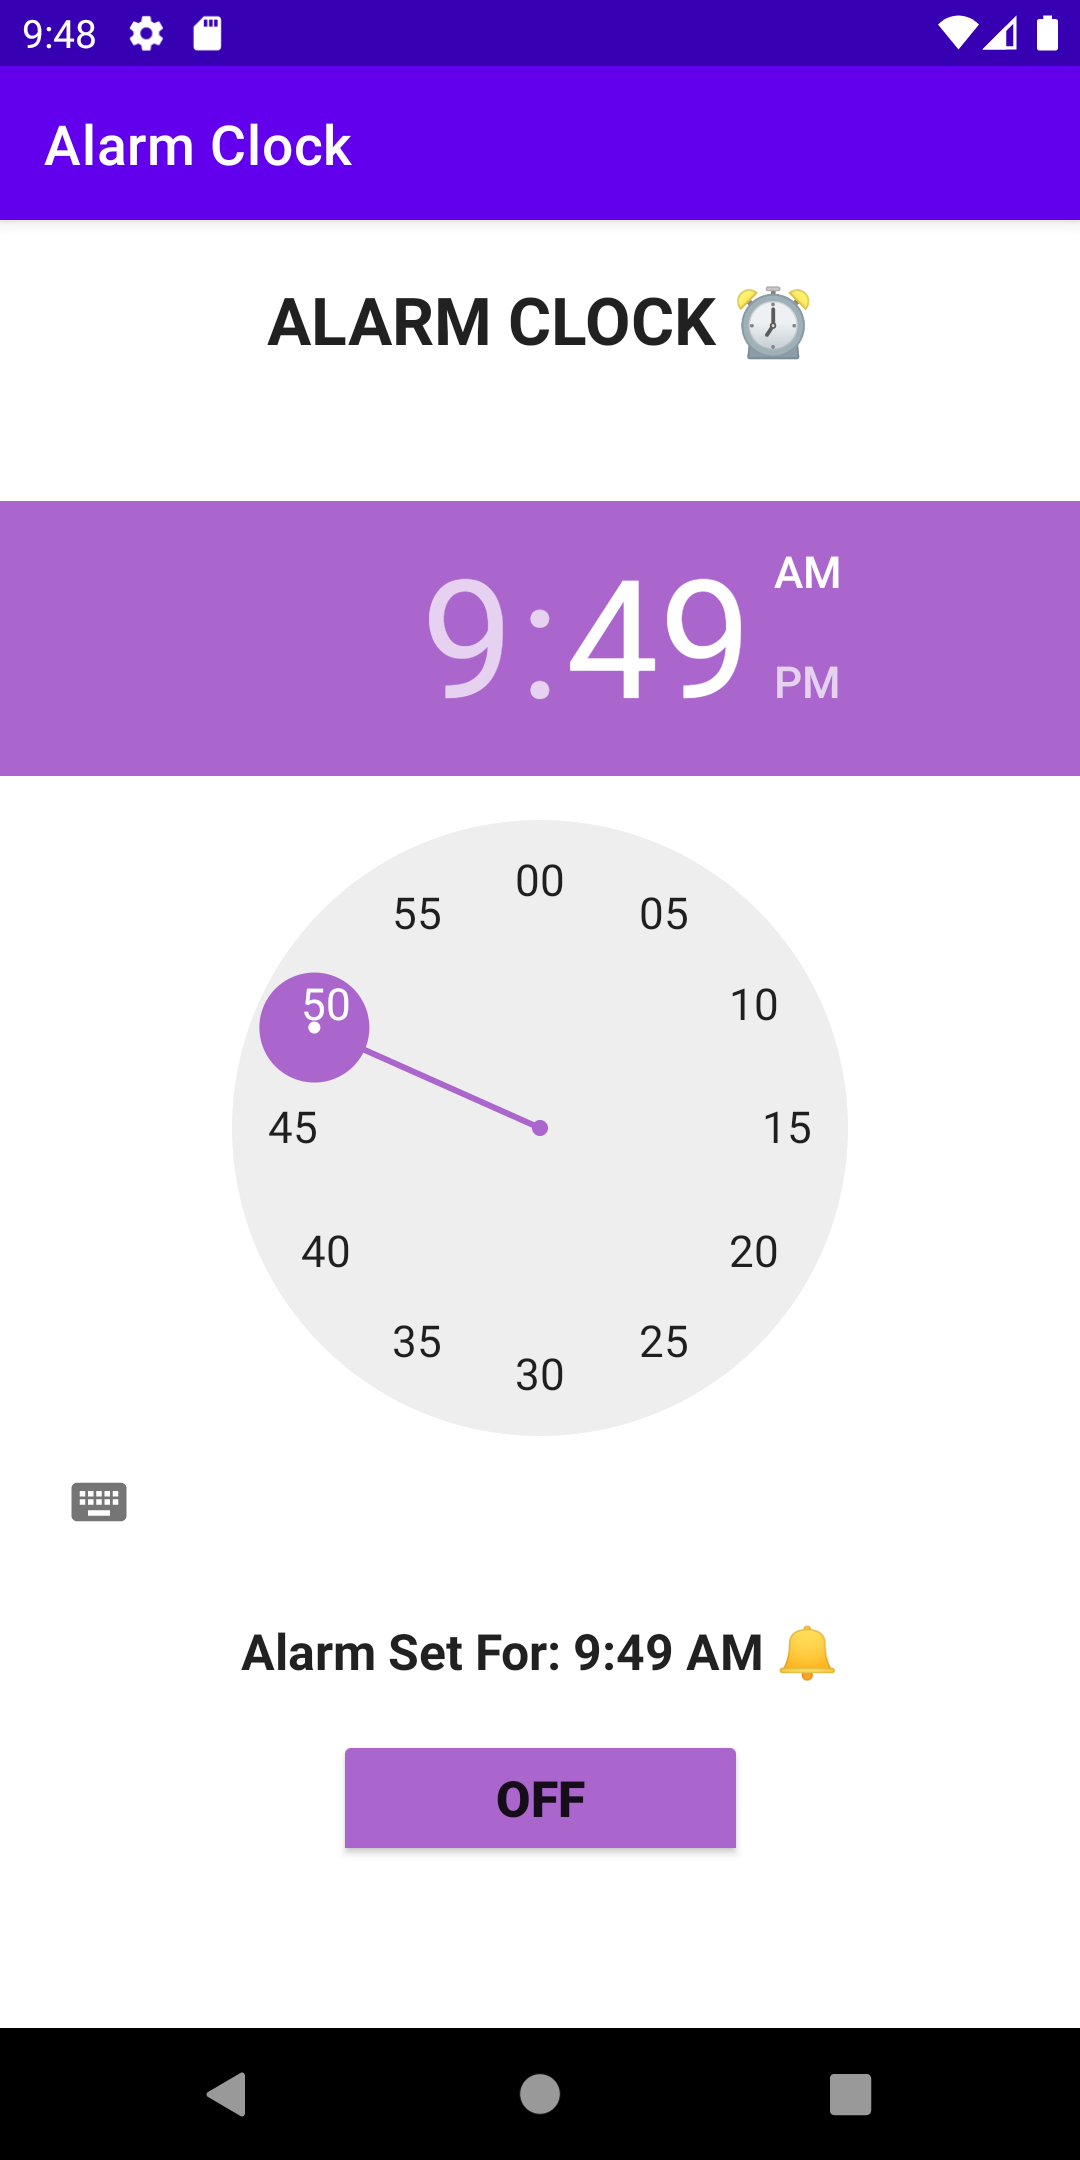
\includegraphics[height=15cm, width=7.3cm]{AlarmClock/Screenshots/Output-2.png}
\end{figure}

%Output
\newpage
\subsection*{\flushleft{Output: Alarm Clock - Alarm Ringing:}}
\begin{figure}[h]
\centering
\caption{Output: Alarm Clock - Alarm Ringing.}
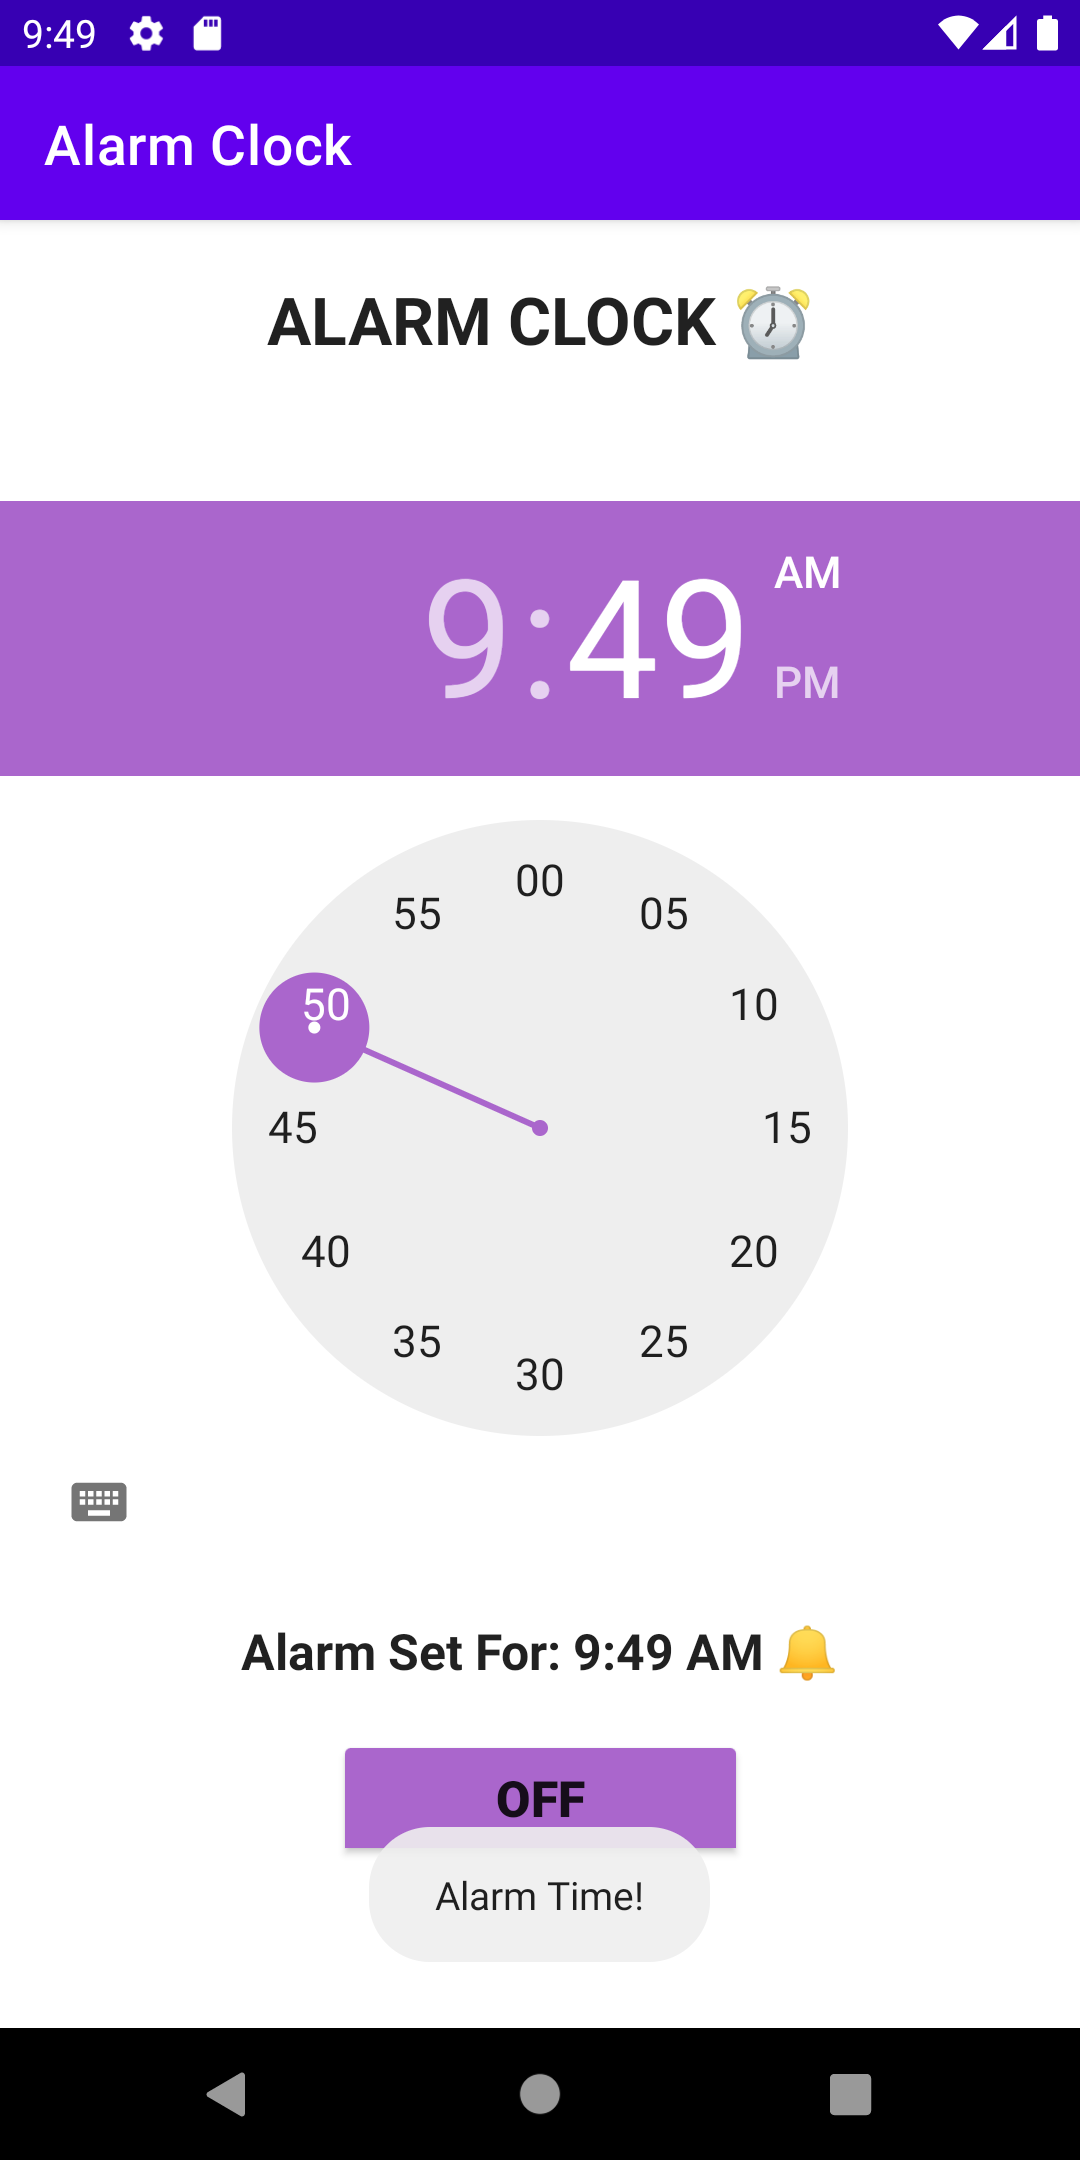
\includegraphics[height=15cm, width=7.3cm]{AlarmClock/Screenshots/Output-3.png}
\end{figure}

%Learning Outcome
\newpage
\subsection*{\flushleft{Learning Outcome:}}
\begin{itemize}
\item I understood how to design a \textbf{Progress Bar} in Android.
\item I understood how to use \textbf{Thread} in Android to handle and update the progress bar's progress value.
\item I understood how Threads work in Android by implementing a \textbf{Runnable} Object and how concurrent execution is handled in the UI using threads.
\item I learnt how to display a \textbf{Progress Dialog} in Android and dismiss it while the main UI was sleeping.
\item I learnt to use a \textbf{ToggleButton} and \textbf{TimePicker} to implement an Alarm Clock in Android.
\item I learnt to use the inbuilt \textbf{AlarmManager} object to set alarms and play a ringtone using the \textbf{Ringtone} object for reminding the user during the time of alarm.
\item I learnt to use \textbf{PendingIntent} and \textbf{Intent} to set the alarm in AlarmManager.
\item I understood how to use \textbf{Log} object for debugging purposes and printing status messages.

\end{itemize}


\end{document}